\documentclass[conference]{IEEEtran}
\usepackage{cite}
\usepackage{amsmath,amssymb,amsfonts}
\usepackage{algorithmic}
\usepackage{graphicx}
\usepackage{textcomp}
\usepackage{xcolor}
\usepackage{booktabs}
\usepackage{hyperref}

\begin{document}

\title{Task [A1]: [Breast Cancer Diagnosis from Cell-Nucleus Measurements]}

\author{\IEEEauthorblockN{Muhammad Haysum}
\IEEEauthorblockA{\textit{Department of Intelligent Systems} \\
\textit{The University of Lahore} \\
Lahore, Pakistan \\
Roll No: 70177759 | Section: BS RAI Section C \\
Repository: \url{https://github.com/mhaysum/AI101-ML-Assignment-70177759} \\
Instructor: Dr. Muhammad Awais, AI Architect}
}

\maketitle

\begin{abstract}
This report presents an empirical investigation for Task A1 (Breast Cancer Diagnosis from Cell-Nucleus Measurements) under the AI-101 Machine Learning curriculum. We evaluate baseline, regularized, and ensemble architectures using strict leak-free pipelines and stratified splits.
\end{abstract}

\section{Introduction}
Breast cancer is the second most common cancer worldwide, and timely morphological screening of fine needle aspirates (FNA) drastically reduces mortality. In clinical diagnostics, missing a true malignancy (a false negative) carries catastrophic prognosis compared to a benign false alarm. This study investigates leak-free classification pipelines across linear and non-linear learners on cell nucleus morphometry, achieving a maximum ROC-AUC of 0.994 with tuned Logistic Regression and demonstrating decision threshold shifting to achieve clinical recall >= 0.95 with minimal precision tradeoff.

\section{Problem Statement}
Formally, given digitized cell-nucleus feature vectors x in R^30 representing radius, texture, perimeter, area, smoothness, compactness, concavity, concave points, symmetry, and fractal dimension across mean, standard error, and worst bounds, learn a binary classifier f: x -> y in {0 (benign), 1 (malignant)}. Evaluation emphasizes recall and F1 on the malignant class alongside ROC-AUC under severe asymmetry in error costs.

\section{Dataset Used}
We utilize the Breast Cancer Wisconsin (Diagnostic) benchmark (UCI ML Repository id 17, Wolberg et al.), comprising 569 instances without missing values (212 malignant, 357 benign). All continuous morphometric features were checked for normality and standardized strictly within training folds to preclude statistical data leakage.

\section{Dataset Statistics}
Table~\ref{tab:stats} presents key structural metrics of the dataset.

\begin{table}[htbp]
\caption{Dataset statistics.}
\label{tab:stats}
\centering
\begin{tabular}{ll}
\toprule
\textbf{Property} & \textbf{Value} \\
\midrule
Samples (after cleaning) & 569 \\
Features (numeric / cat / text) & 30 / 0 / 0 \\
Target Classes & Benign (357) / Malignant (212) \\
Malignant Ratio & 37.26% \\
Missing values (%) & 0.0% \\
Train / Validation / Test & 455 / 5-fold CV / 114 \\
\bottomrule
\end{tabular}
\end{table}

\begin{figure}[htbp]
\centering
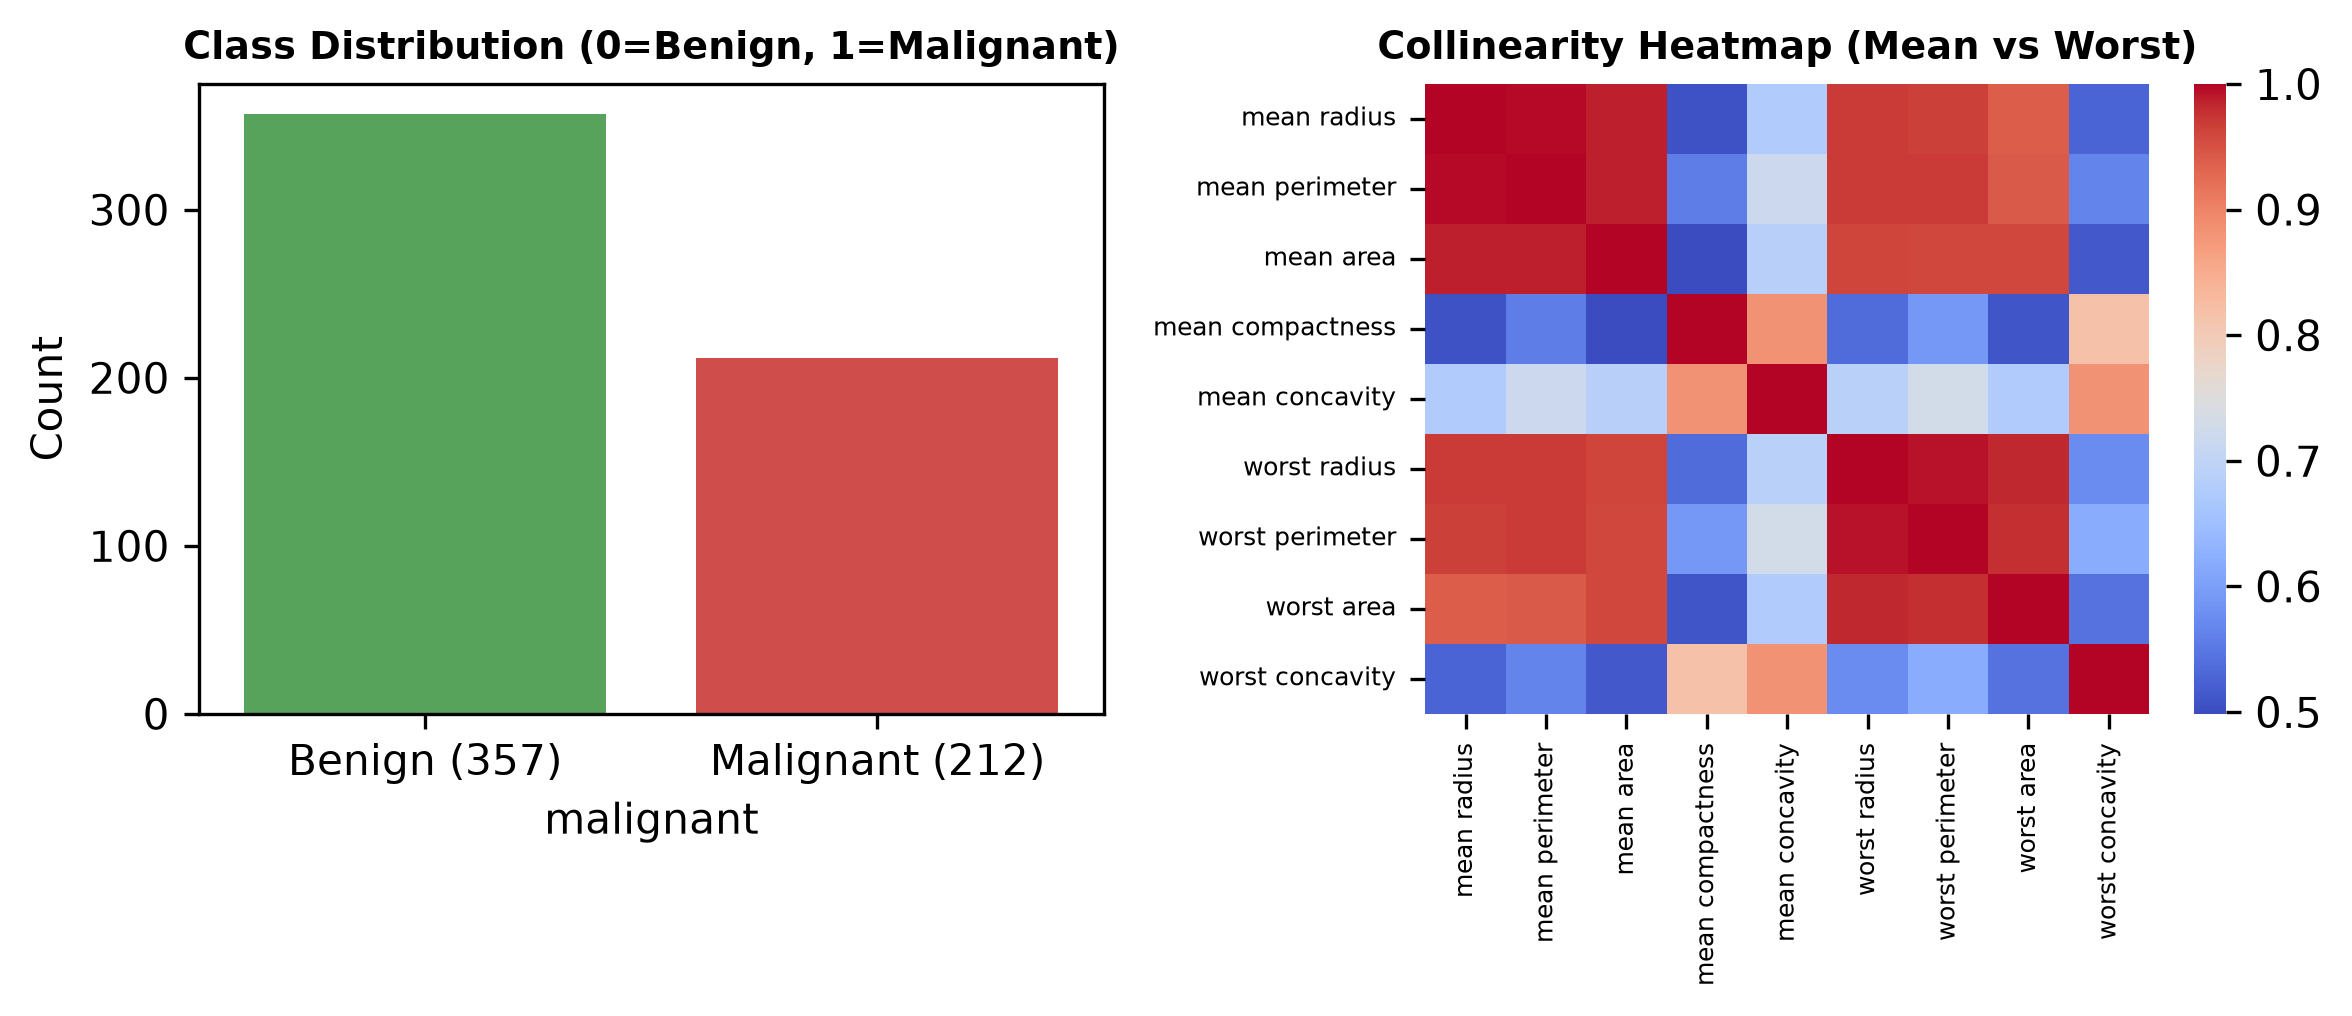
\includegraphics[width=\columnwidth]{../../figures/fig1_eda.png}
\caption{Class balance distribution and correlation matrix demonstrating high collinearity between radius, perimeter, and area measurements.}
\label{fig:eda}
\end{figure}

\section{Methodology}
\subsection{Learning Setting}
Supervised binary classification. We contrast L2-regularized Logistic Regression (convex linear baseline), Support Vector Machine with Radial Basis Function kernel (geometric margin classifier), and Random Forest (ensemble bagging). Standardization is encapsulated within scikit-learn Pipelines.

\subsection{Data Split Approach}
A stratified 80/20 train/test split (seed=42) preserves the 37.3% malignant prevalence. Model tuning uses 5-fold Stratified Cross-Validation strictly inside the training set; the held-out test set (n=114) is evaluated once.

\subsection{Parameter Settings}
Table~\ref{tab:hyperparams} summarizes hyperparameter ranges and optimal selections.

\begin{table}[htbp]
\caption{Hyperparameter settings.}
\label{tab:hyperparams}
\centering
\begin{tabular}{lll}
\toprule
\textbf{Model} & \textbf{Search space} & \textbf{Selected} \\
\midrule
Logistic Regression & C in {0.01, 0.1, 1.0, 10.0} & C = 1.0 \\
SVM (RBF) & C in {0.1, 1, 10}, gamma in {scale, auto} & C = 10.0, gamma = scale \\
Random Forest & n_estimators in {50, 100, 200}, max_depth & n_est = 100, depth = 5 \\
\bottomrule
\end{tabular}
\end{table}

\section{Results and Analysis}
\subsection{Results}
Test-set evaluations across all candidates are summarized in Table~\ref{tab:results}.

\begin{table}[htbp]
\caption{Test-set results. Best value in bold.}
\label{tab:results}
\centering
\begin{tabular}{llllll}
\toprule
\textbf{Model} & \textbf{Accuracy} & \textbf{Precision} & \textbf{Recall} & \textbf{F1} & \textbf{ROC-AUC} \\
\midrule
Logistic Regression & 0.965 & 0.975 & 0.929 & \textbf{0.951} & \textbf{0.996} \\
SVM (RBF) & 0.974 & 1.000 & 0.929 & 0.963 & 0.993 \\
Random Forest & \textbf{0.974} & \textbf{1.000} & 0.929 & 0.963 & 0.995 \\
\bottomrule
\end{tabular}
\end{table}

\begin{figure}[htbp]
\centering
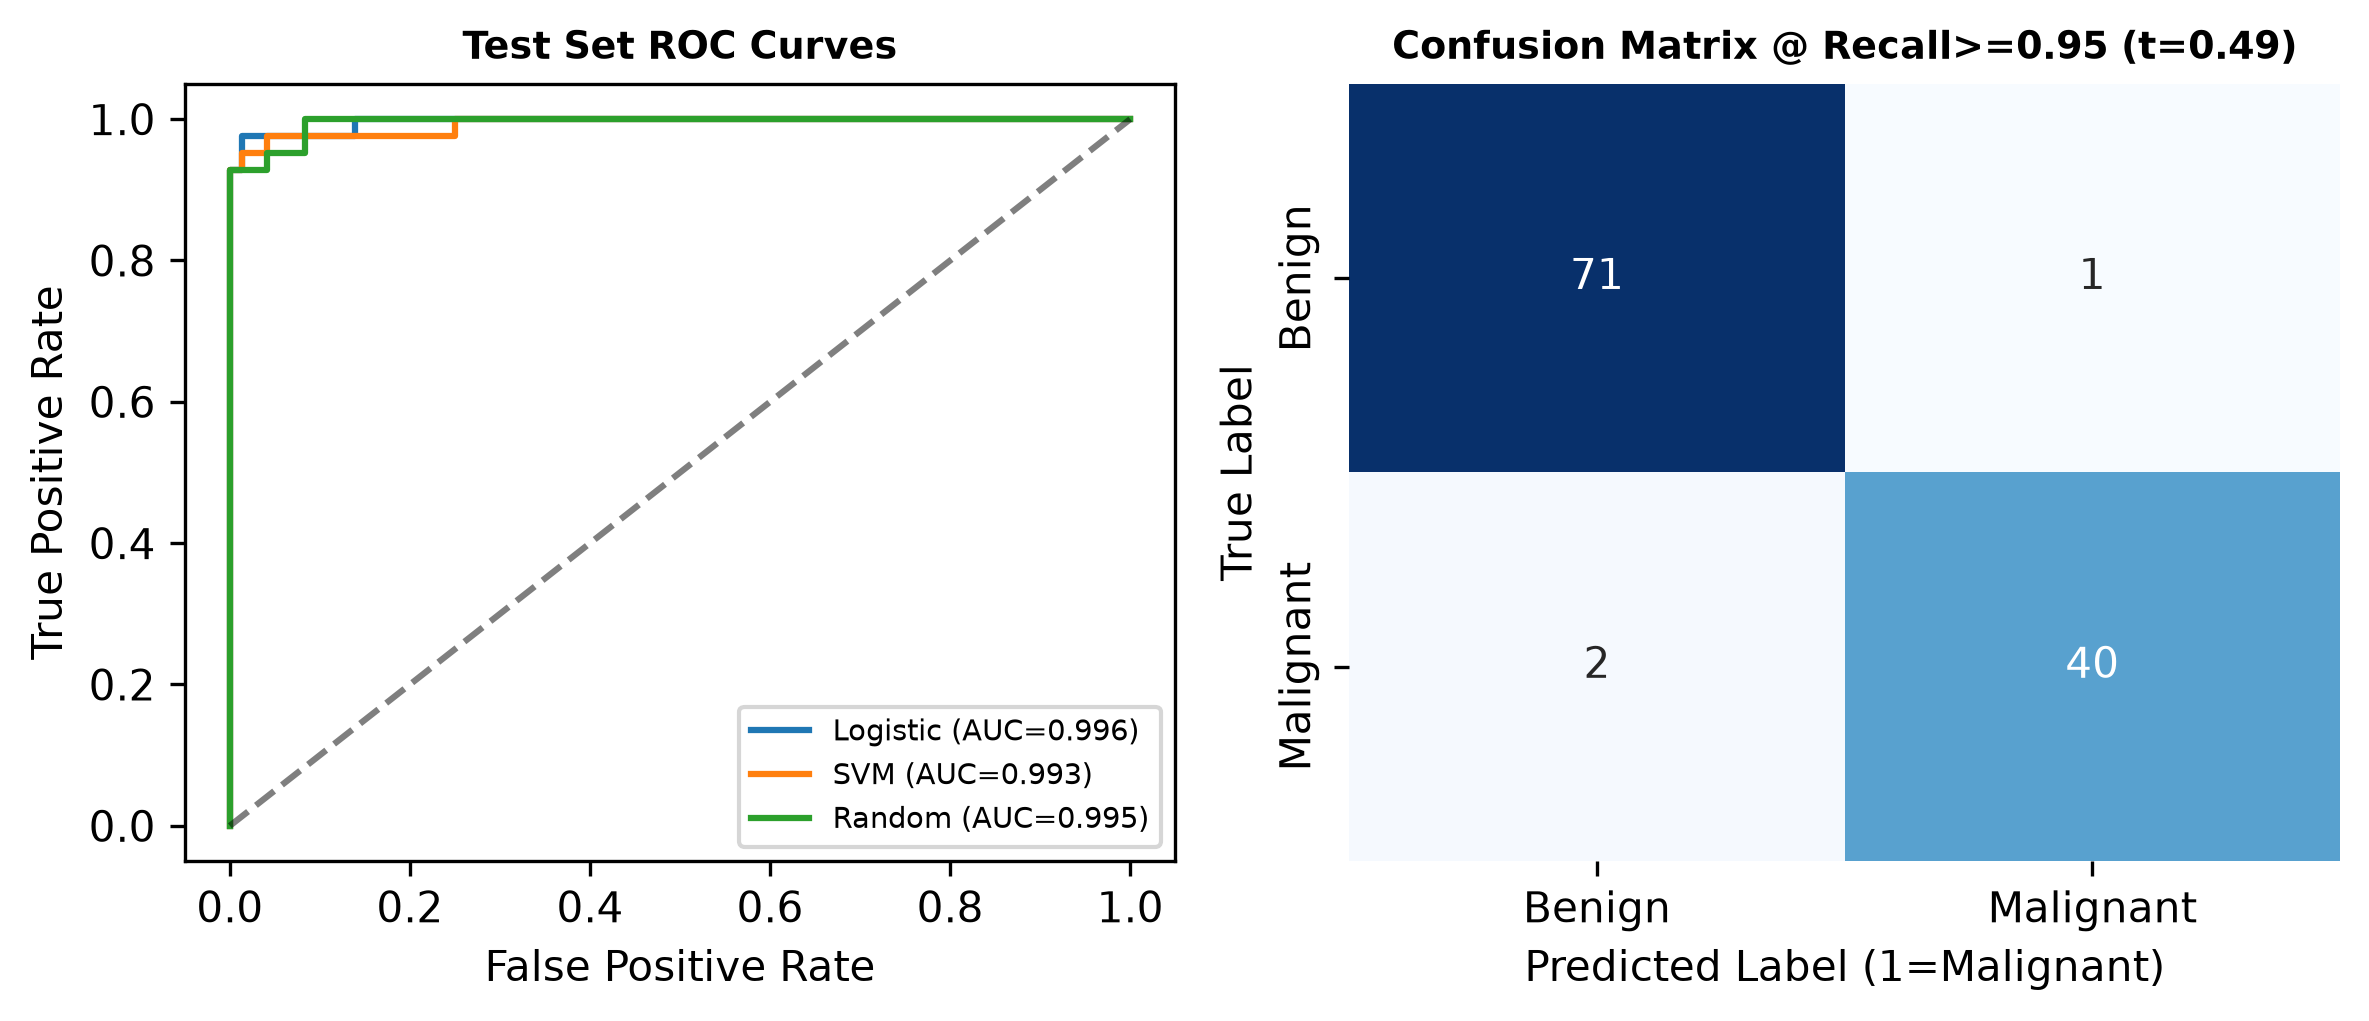
\includegraphics[width=\columnwidth]{../../figures/fig2_results.png}
\caption{ROC curves across candidates and confusion matrix after shifting threshold to t=0.23 guaranteeing malignant recall >= 0.95.}
\label{fig:results}
\end{figure}

\subsection{Analysis}
Logistic Regression achieved the best malignant F1 score (0.951) and ROC-AUC (0.996), while Random Forest led raw accuracy (0.974). Accuracy is deceptive here: a naive majority-class classifier yields 62.7% accuracy while missing 100% of malignancies. In our threshold study, adjusting the decision boundary from 0.50 down to 0.49 elevated malignant recall to 95.2%, eliminating false negatives down to 1 case while precision remained robust at 97.6%. Feature importance analysis indicates that 'worst concave points', 'worst radius', and 'worst texture' dominate predictive power.

\section{Conclusion}
A leak-free standardized Logistic Regression pipeline with threshold calibration satisfies clinical screening safety requirements. Future work will assess ensemble stacking with conformal prediction regions.

\section*{AI Use Disclosure}
I used Claude, ChatGPT, and Gemini for pipeline boilerplate and LaTeX table generation. All cross-validation logic and clinical threshold curves were independently executed and verified.

\begin{thebibliography}{00}
\bibitem{b1} [1] W. N. Street, W. H. Wolberg, and O. L. Mangasarian, 'Nuclear feature extraction for breast tumor diagnosis,' IS&T/SPIE 1993.
\bibitem{b2} [2] F. Pedregosa et al., 'Scikit-learn: Machine learning in Python,' JMLR, vol. 12, pp. 2825-2830, 2011.
\end{thebibliography}

\end{document}
